\section{\normalsize Диффузия: закон Фика, коэффициент диффузии, уравнение диффузии. Коэффициент диф	фузии в газах.}
Средняя скорость течения газа определяется формулой: $\textbf{u}=\dfrac{1}{n}\sum_{i}^{}\textbf{v}_i$.

Плотность потока частиц: $\textbf{j}=n\textbf{u}$

\textbf{Диффузия} --- неравновесный процесс пространственного перераспределения компонент смеси относительно друг друга, обусловленный случайным (тепловым) движением молекул.

Рассмотрим бинарные смеси. Пусть имеется бинарная смесь с плотностью  $n=n_1+n_2$, $n_1, n_2$ --- плотности компонентов, $[n]$=частиц/см$^3$.

\textbf{Концентрации или относительные концентрации:} $c_1=\dfrac{n_1}{n}$, $c_2=\dfrac{n_2}{n}$, $c_1+c_2=1$.

Пусть средняя скорость течения газа \textbf{u}=0, а диффузия осуществляется вдоль оси х. Плотности потоков компонентов смеси даются \textbf{законом Фика:}

$j_1=-Dn\dfrac{dc_1}{d_x}$, $j_2=-Dn\dfrac{dc_2}{d_x}$ => $j_1+j_2=0$.

То есть диффузия не меняет плотности среды, но приводит к изменению относительных концентраций компонент.

\textbf{Коэффициентом диффузии} называется величина D. [D]=см$^2$/c.

Если $n=n_1+n_2=const$, то $j_1=-D\dfrac{dn_1}{dx}$, $j_2=-D\dfrac{dn_2}{dx}$.

Если скорость течения газа ненулевая, то добавляются слагаемые, учитывающие течение газа как целого: $j_1=-Dn\dfrac{dc_1}{d_x}+nc_1u$, $j_2=-Dn\dfrac{dc_2}{d_x}+nc_2u$, $j=j_1+j_2=nu$.

Для трехмерного случая: 

$\textbf{j}_1=-Dngradc_1+nc_1\textbf{u}$,\hspace{0.5 cm} $\textbf{j}_2=-Dngradc_2+nc_2\textbf{u}$ \hspace{0.5 cm}
=>\hspace{0.5 cm} $\textbf{j}=\textbf{j}_1+\textbf{j}_2=n\textbf{u}$

\textbf{Уравнение диффузии}

Рассмотрим поток частиц одного сорта вдольоси х. В объеме $dV=dSdx$ число частиц $dN_1=n_1dV$, где $n_1=т_1(x,t)$ --- их число в единице объема в момент времени t.

Пусть $j_1=j_1(x,t)$--- плотность потока рассматриваемых частиц. Число частиц,поступивших в объем dV в единицу времени: $(j_1(x,t)-j_1(x+dx,t))dS=-\dfrac{\partial j_1}{\partial x}dV$ 

Эта величина есть скорость изменения числа частиц в выделенном объеме dV, то есть 
$\partial(dN_1)/\partial t$.

Таким образом, уравнение баланса: \hspace{1 cm} $\dfrac{\partial n_1}{\partial t}+\dfrac{\partial j_1}{\partial x}=0$

Пусть средняя скорость течения газа u=0. Из закона Фика: $j_1=-Dn\dfrac{dc_1}{d_x}$, $n_1=nc_1$.

\begin{wrapfigure}[4]{l}{0.35\linewidth} 
	\vspace{-5ex}
	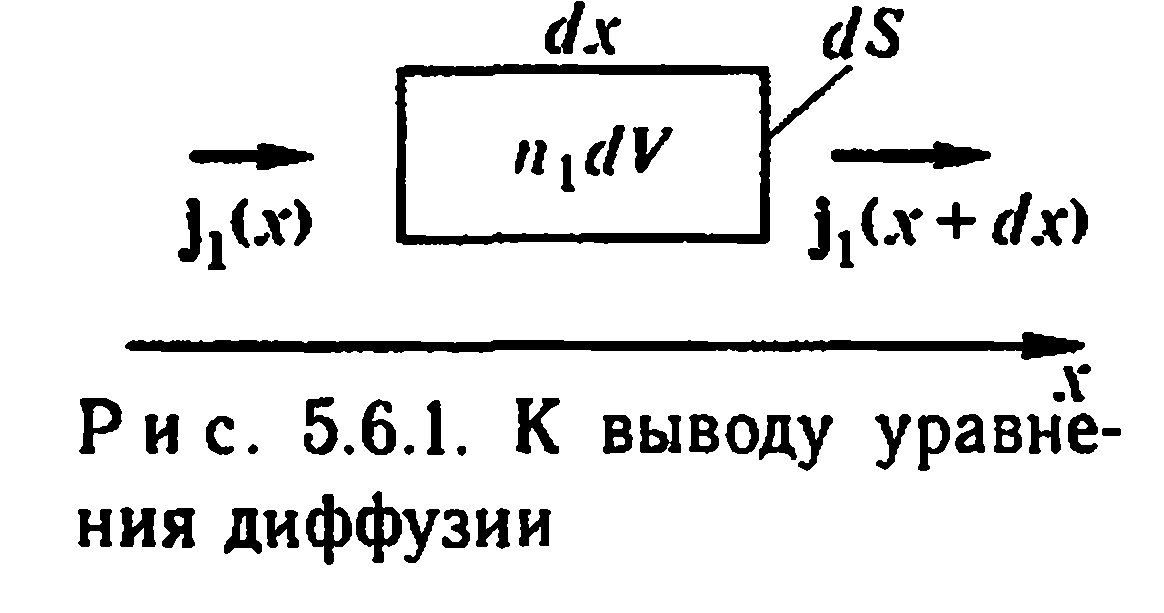
\includegraphics[width=\linewidth]{urdif}
	
	
\end{wrapfigure}

\textbf{Уравнение диффузии:} \hspace{1 cm} $\dfrac{\partial(nc_1)}{\partial t}=\dfrac{\partial}{\partial x}\left(nD\dfrac{\partial c_1}{\partial x}\right)$.

Если n=const, то: $\dfrac{\partial(n_1)}{\partial t}=\dfrac{\partial}{\partial x}\left(D\dfrac{\partial n_1}{\partial x}\right)$.

В трехмерном случае: $\dfrac{\partial(nc_1)}{x}=div(D n gradc_1)$.

Пусть средняя скорость течения газа ненулевая.

Если $j_1=n\left(-D\dfrac{\partial c_1}{\partial x}+c_1u\right)$, то $\dfrac{\partial(nc_1)}{\partial t}+\dfrac{\partial(nc_1u)}{\partial x}=\dfrac{\partial}{\partial x}\left(nD\dfrac{\partial c_1}{\partial x}\right)$.

В трехмерном случае: $\dfrac{\partial(nc_1)}{\partial t}+div(nc_1u)=div(nDgradc_1)$ --- \textbf{уравнение диффузии со сносом(конвекция)}.

Для второй компоненты:  $\dfrac{\partial(nc_2)}{\partial t}+div(nc_2u)=div(nDgradc_2)$.

Сложив последние два равенства и учитывая $c_1+c_2=1$ получим: $\dfrac{\partial n}{\partial t}+div\textbf{j}=0$, $\textbf{j}=n\textbf{u}$---\textbf{уравнение непрерывности}.

\textbf{Коэффициент диффузии}

\begin{wrapfigure}[7]{l}{0.35\linewidth} 
	\vspace{-5ex}
	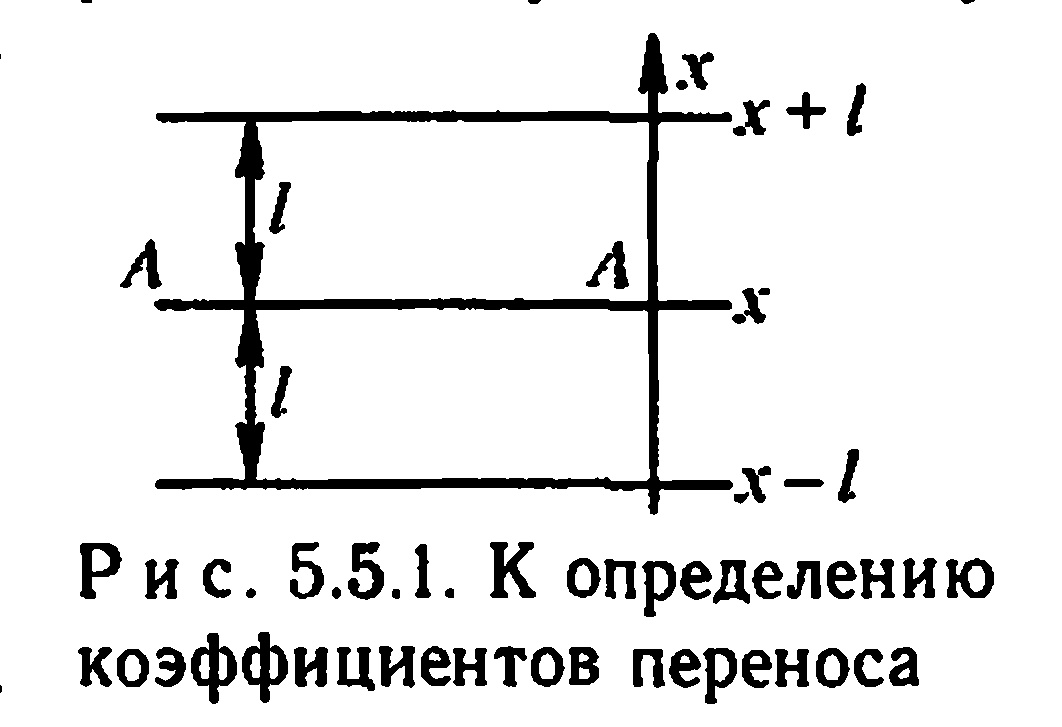
\includegraphics[width=\linewidth]{koef}
	
\end{wrapfigure}

Число молекул, проходящих вверх за время свободного пробега $\tau$ через единицу площади в плоскоти с координатой х: $N_1=\dfrac{1}{6}n(x-l)\overline{\mathit{v}}\tau$ и вниз $N_2=\dfrac{1}{6}n(x+l)\overline{\mathit{v}}\tau$

$\mathit{v}$--- средняя тепловая скорость, а l --- длина свободного пробега.

По определению диффузионного потока $j=\dfrac{N_1-N_2}{\tau}\simeq$

$\simeq-\dfrac{1}{3}\overline{\mathit{v}}l\dfrac{dn}{dx}$ => $D=\dfrac{1}{3}\overline{\mathit{v}}l$

Так как $l=1/(n\sigma)$,\hspace{0.5 cm} $n\sim P/T$,\hspace{0.5 cm} $\overline{\mathit{v}}\sim\sqrt{T/m}$, то \hspace{0.5 cm}
$D\sim\dfrac{T^{3/2}}{P\sqrt{m}}$.